\begin{figure}[htbp]\centering
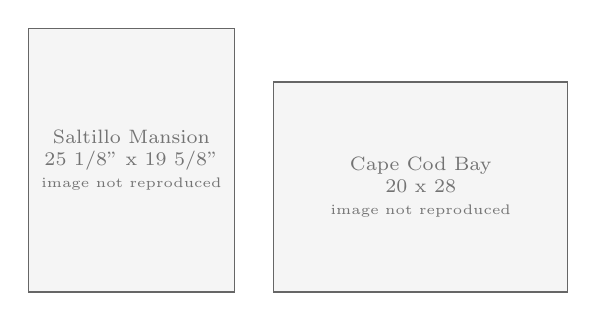
\begin{tikzpicture}
\draw[fill=black!4,draw=black!60,line width=0.5pt] (0,0) rectangle (2.6166666666666667,3.35);
\node[align=center,text=black!55,font=\scriptsize] at (1.3083333333333333,1.675) {Saltillo Mansion\\25 1/8" x 19 5/8"\\\tiny image not reproduced};
\draw[fill=black!4,draw=black!60,line width=0.5pt] (3.1166666666666667,0) rectangle (6.85,2.6666666666666665);
\node[align=center,text=black!55,font=\scriptsize] at (4.983333333333333,1.3333333333333333) {Cape Cod Bay\\20 x 28\\\tiny image not reproduced};
\end{tikzpicture}
\caption{\textbf{Saltillo Mansion}, watercolour, August 1943, 25 1/8" x 19 5/8" as the leaf writes it (Book III, leaf 101, ref 17944). The Metropolitan Museum of Art, 45.157.2: \url{https://www.metmuseum.org/art/collection/search/488165}. \textbf{Cape Cod Bay}, watercolour, 1965; the last work leaf photographed, 20 x 28 as the leaf writes it (Book III, leaf 125, ref 16620). Whitney Museum of American Art, work 6829: \url{https://whitney.org/collection/works/6829}. Scale: sixty inches to eight centimetres; an upright Mexican sheet of 1943 beside a Cape watercolour of 1965 on the full imperial sheet. The frames are drawn to the proportions of the size in Edward Hopper's hand; the images are not reproduced here and can be seen at the museums' own pages. Drawn by Claude Fable~5.1, 13 September 2026, from the transcriptions and \texttt{works.json} (2026-09-13).}\label{fig:watercolours}
\end{figure}
